\documentclass{article} % For LaTeX2e
\usepackage{nips15submit_e,times}
\usepackage{hyperref}
\usepackage{graphicx}
\usepackage{hyperref}
\usepackage{url}
\usepackage{times}
\usepackage{epsfig}
\usepackage{graphicx}
\usepackage{amsmath}
\usepackage{amssymb}
\usepackage{multirow}
\usepackage{caption} 
\usepackage{url}
%\documentstyle[nips14submit_09,times,art10]{article} % For LaTeX 2.09

\title{Recurrent Batch Normalization}

\author{
Me \\
\And
Nicolas \\
\And
C\'esar \\
\And
Aaron
\texttt{email} \\
}

\newcommand{\fix}{\marginpar{FIX}}
\newcommand{\new}{\marginpar{NEW}}

%\nipsfinalcopy % Uncomment for camera-ready version

\usepackage{amsfonts}
\usepackage{amsmath}

\newcommand{\vect}[1]{\mathbf{#1}}
\newcommand{\mat}[1]{\mathbf{#1}}
\newcommand{\act}{f}
\newcommand{\ewprod}{\odot}
\newcommand{\reals}{\mathbb{R}}
\newcommand{\given}{\vert}

\bibliographystyle{plain}

\begin{document}

\maketitle

\begin{abstract}
We propose a reparameterization of LSTM that brings the benefits of batch normalization to recurrent neural networks.
Empirical results show faster convergence and improved generalization on classification, language modeling and speech transcription tasks.
\end{abstract}

\section{Introduction}

Training deep neural networks by gradient descent is hard due in large part to pathological curvature in the objective function.
Approaches to alleviating this problem divide naturally into two categories: smarter optimization algorithms such as
Hessian-Free~\cite{hessianfree} and various approximations to natural gradient~\cite{amari} proposed in~\cite{ollivier} and~\cite{KFAC},
and model reparameterizations~\cite{efficientbackprop}~\cite{raiko}~\cite{naturalneuralnetworks}.

Batch normalization~\cite{batchnorm} is a recently proposed reparameterization that [actually works].
It involves normalizing unit preactivations in order to make their distributions easier to control.
This greatly improves the training dynamics of deep feedforward neural networks, leading to faster convergence and better generalization.

However, applying batch normalization in recurrent neural networks (RNNs) has proven to be challenging.
It has found limited use in stacked RNNs, where the normalization is applied ``vertically'', i.e. to the input of each RNN~\cite{cesar}~\cite{baidu}, but not ``horizontally'' between timesteps.
Indeed, normalizing horizontally -- where RNNs are deepest and would most benefit from the reparameterization -- was thought to be unhelpful until now.

Recently, a related technique called weight normalization~\cite{weightnorm} was introduced, which has a similar effect to batch normalization yet might be easier to carry over to the recurrent setting.
[also normprop]
However to our knowledge none of these schemes have yet been transferred to RNNs.

In this paper, we demonstrate how batch normalization can be used in RNNs to speed up optimization and improve generalization.
Section~\ref{sec:prerequisites} introduces RNNs and batch normalization in detail.
In Section~\ref{sec:recurrent-batch-normalization} we discuss batch normalization in the recurrent setting.
We show in Section~\ref{sec:experiments} our evaluations of the proposed reparameterization on a variety of tasks.

\section{Prerequisites}
\label{sec:prerequisites}

\subsection{Recurrent neural networks}

Given an input sequence $\mat{X} = ( \vect{x}_1, \vect{x}_2, ... \vect{x}_T )$,

\begin{align}
\vect{h}_t = \mathrm{tanh}(
  \mat{W}_h \vect{h}_{t-1} +
  \mat{W}_x \vect{x}_t +
  \vect{b})
\end{align}

where $\mat{W}_h \in \reals^{d_h \times d_h},
       \mat{W}_x \in \reals^{d_x \times d_h},
       \vect{b} \in \reals^{d_h}$
  and the initial state $\vect{h}_0 \in \reals^{d_h}$
  are model parameters.

RNNs are popular in sequence modeling tasks, as they naturally apply to variable-length sequences.

Being dynamical systems, RNNs can exhibit chaotic behavior, and indeed controlling their dynamics is an area of active research.
Training RNNs by gradient descent is notoriously difficult as we need to not only control the dynamics of the forward-propagated activations but also those of the back-propagated gradient.
This leads to the much-studied problem of vanishing and exploding gradients~\cite{bengiolongterm}~\cite{pascanudifficulty}.

There exist a number of variants of the basic RNN given above, some specifically designed to address the problem of vanishing and exploding gradients, such as the Long Short-Term Memory (LSTM) unit~\cite{lstm} and Unitary RNNs~\cite{urnn}.  We will focus on LSTM, with recurrent transition given by

\begin{align}
\left(\begin{array}{ccc}
\tilde{\vect{f}}_t \\
\tilde{\vect{i}}_t \\
\tilde{\vect{o}}_t \\
\tilde{\vect{g}}_t
\end{array}\right)
 &=
 \mat{W}_h \vect{h}_{t-1} +
 \mat{W}_x \vect{x}_t +
 \vect{b}
\\
\vect{c}_t &= \sigma(\tilde{\vect{f}}_t) \ewprod \vect{c}_{t-1} +
              \sigma(\tilde{\vect{i}}_t) \ewprod \mathrm{tanh}(\tilde{\vect{g}_t}) \\
\vect{h}_t &= \sigma(\tilde{\vect{o}}_t) \ewprod \tanh(\vect{c}_t)
\end{align}

where $\vect{W}_h \in \reals^{d_h \times 4 d_h}, \vect{W}_x \reals^{d_x \times 4 d_h}, \vect{b} \in \reals^{4 d_h}$ and the initial states $\vect{c}_0, \vect{h}_0 \in \reals^{d_h}$ are model parameters.
The $\ewprod$ operator denotes the elementwise product.

Intuitively, LSTM improves on the basic RNN in two ways.
First, it has an additional recurrent \emph{cell} state $\vect{c}_t$ whose recurrence is nearly linear, which allows gradient to flow more easily.
Second, communication between this state and $\vect{h}_t$ and $\vect{x}_t$ is controlled by the gates $\vect{f}_t$, $\vect{i}_t$ and $\vect{o}_t$.
With these gates, the model can control what to forget and what to remember.

\subsection{Batch normalization}

Batch normalization~\cite{batchnorm} is a simple reparameterization applied to neural network preactivations in order to make their distributions easier to control.
The batch normalizing transform is as follows:

\begin{align}
\mathrm{BN}(\vect{h}; \gamma, \beta) =
  \beta + \gamma
  \frac{\vect{h} -   \widehat{\mathbb{E}}(\vect{h})}
       {       \sqrt{\widehat{\mathrm{Var }}(\vect{h}) + \epsilon}}
\end{align}

where $\vect{h} \in \reals^d$ is the vector of (pre)activations to be normalized, $\gamma \in \reals^d, \beta \in \reals^d$ are model parameters that determine the mean and standard deviation of the normalized activation, and $\epsilon \in \reals$ is a regularization hyperparameter.

At training time, the statistics $\mathbb{E}(\vect{h})$ and $\mathrm{Var}(\vect{h})$ are estimated by the sample mean and sample variance of the current minibatch.
This allows for backpropagation through the statistics, preserving the convergence properties of stochastic gradient descent.
During inference, the statistics are typically estimated based on the entire training set, to produce a deterministic prediction.

Batch normalizing some hidden layer's activation ensures that its mean and variance are determined only by the $\beta$ and $\gamma$ parameters, and not by the parameters of any layer below it.
Applying this on every layer effectively decouples each layer's parameters from those of other layers, leading to a better-conditioned optimization problem.
Deep neural networks trained with batch normalization converge significantly faster and generalize better.

\section{Recurrent batch normalization}
\label{sec:recurrent-batch-normalization}

A RNN can be ``unrolled'' and viewed as a feedforward neural network.
This view suggests that the success of batch normalization in feedforward networks should carry over to the recurrent setting.
However, unrolled RNNs differ from true feedforward networks in several important respects that complicate the application of batch normalization.

\begin{itemize}
\item
The parameters in an unrolled RNN are shared across layers.
This suggests that the statistics used for normalization should be shared as well.
However, we have found that estimating the statistics independently at each timestep works best.
With batch normalization, the activations rapidly converge to a stationary distribution (cf. a figure), so independent estimation does not hurt performance.
Indeed, we find that sharing statistics does hurt performance, as the distribution of activations during the first few timesteps is very different from the stationary distribution.
\\ \item
The depth depends on the length of the input sequence $\mat{X} = (\vect{x}_t)$, which is typically not constant.
This poses a problem if we want to estimate the population statistics for different timesteps independently.
However, thanks to the stationarity of the activation distribution (cf. that figure) we can use the estimates of earlier timesteps for later timesteps.
For our experiments we estimate the population statistics separately for each timestep $1, \ldots, T_{max}$ where $T_{max}$ is the length of the longest training sequence.
When at test time we need to generalize beyond $T_{max}$, we use the population statistic of time $T_{max}$ for all time steps following it.

[there is an annoying little detail here: there may be only a single example with length T, and so the population statistic is highly unreliable. in this case i would take an earlier population statistic instead, the exact choice determined by validation. how do we explain this concisely?]
[additionally, we haven't actually dealt with variable-length training sequences yet. this is another technicality that's easily hacked around but people will want to know i guess.]
\\ \item
There is three-way interaction; each layer receives as input not just the activations of the layer below it but also the next element of the input sequence.
We find that we need to normalize these terms separately before adding them up.
This gives the model better control over the relative contribution of the terms.
\\ \item
The initial states $\vect{h}_0$ are independent of the input and thus have zero variance.
This problem is exacerbated in unnatural data such as MNIST and various pathological tasks, where some features are constant across the data.
In the sequential MNIST task in particular, the variance is typically exactly zero for the first hundred or so time steps, as the upper pixels are almost always black.
Normalizing these zero-variance activations involves division by a very small number at many timesteps, which causes the gradient to explode.
We work around this by injecting noise into the initial hidden states.
Although the normalization amplifies the noise to signal level, we find that it does not hurt performance compared to data-dependent ways of initializing the hidden states.
[but is that an artifact of classification at the end?]
\\ \item
Unrolled RNNs are usually much deeper than typical feedforward networks.
Rather than normalizing activations to have standard deviation 1, we normalize to standard deviation 0.1.
This avoids saturating the nonlinearities and enables better flow of gradients.
Indeed, we found that normalizing to unit variance caused the gradient to vanish rapidly.
[yet explode in LSTM...]
\end{itemize}

\subsection{Batch-normalized LSTM}

We introduce the batch normalizing transform $\mathrm{BN}(\cdot; \gamma, \beta)$ into the LSTM transition as follows:

\begin{align}
\left(\begin{array}{ccc}
\tilde{\vect{f}}_t \\
\tilde{\vect{i}}_t \\
\tilde{\vect{o}}_t \\
\tilde{\vect{g}}_t
\end{array}\right)
 &=
 \mathrm{BN} (\mat{W}_h \vect{h}_{t-1}; \gamma_h, \beta_h) +
 \mathrm{BN} (\mat{W}_x \vect{x}_t    ; \gamma_x, \beta_x) +
 \vect{b}
\\
\vect{c}_t &= \sigma(\tilde{\vect{f}}_t) \ewprod \vect{c}_{t-1} +
              \sigma(\tilde{\vect{i}}_t) \ewprod \mathrm{tanh}(\tilde{\vect{g}_t}) \\
\vect{h}_t &= \sigma(\tilde{\vect{o}}_t) \ewprod \tanh(
 \mathrm{BN} (\vect{c}_t; \gamma_c, \beta_c)
)
\end{align}

Note how we normalize the recurrent term $\mat{W}_h \vect{h}_{t-1}$ and the input term $\mat{W}_x \vect{x}_t$ separately.
This allows the model to control the contribution of the two independently using $\gamma_h$ and $\gamma_x$.
To avoid unnecessary redundancy we set $\beta_h = \beta_x = \vect{0}$, instead relying on the pre-existing parameter vector $\vect{b}$ to account for both biases.

In order to leave the LSTM dynamics intact, we do not introduce batch normalization into the recurrence of the cell states.

During training we estimate the statistics needed for batch normalization across the minibatch, and independently for each timestep.
During inference we use estimates obtained by averaging the minibatch estimates both across the training set and across time.

\section{Experiments}
\label{sec:experiments}

\subsection{Sequential MNIST}

\begin{figure}
\center
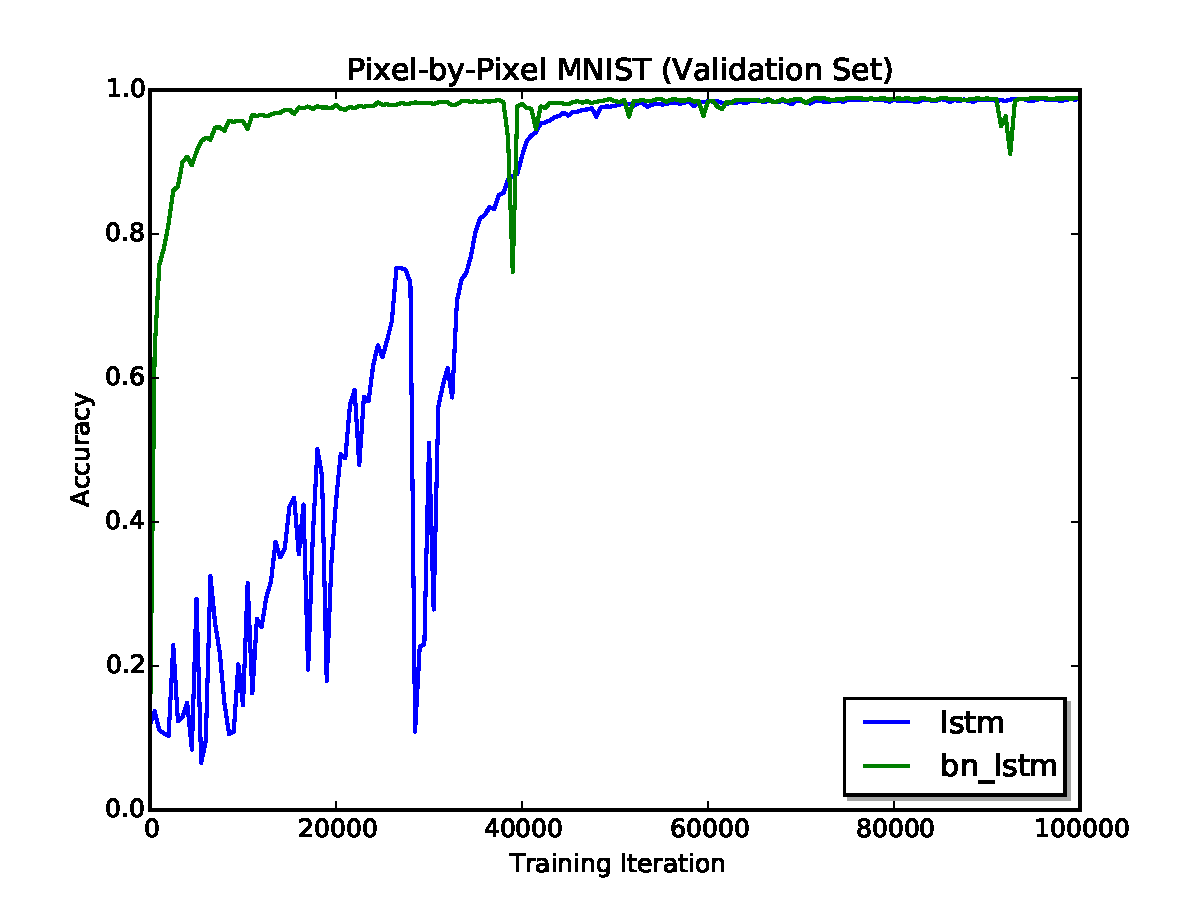
\includegraphics[width=7cm]{figures/unpermuted_valid.pdf}
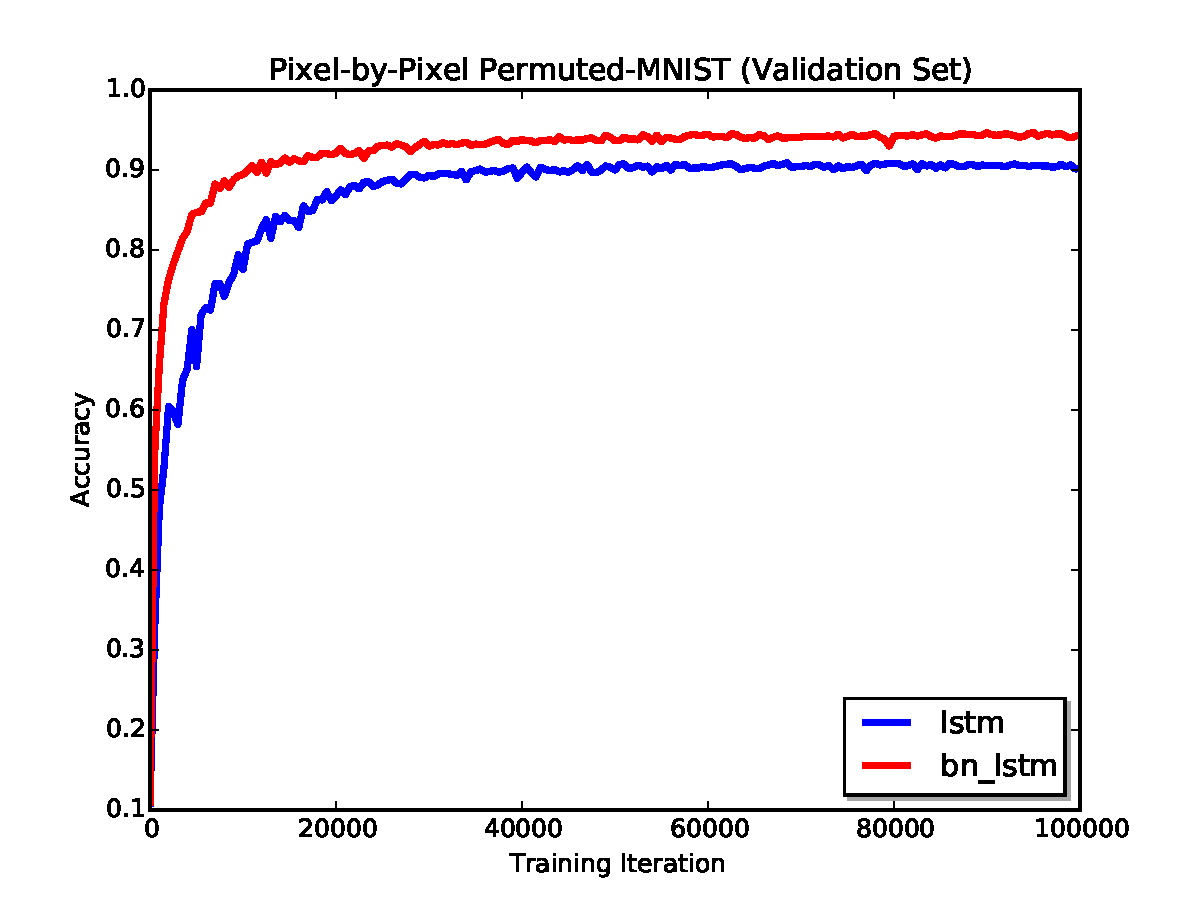
\includegraphics[width=7cm]{figures/permuted_valid.pdf}
\caption{Accuracy on the validation set for the pixel by pixel MNIST classification tasks. The batch-normalized LSTM is able to converge faster relatively to a baseline LSTM.
  Batch-normalized  LSTM also shows some improve generalization on the permuted sequential MNIST that require to preserve long-term memory information.}
\label{fig:seqmnist_valid}
\end{figure}


\begin{table}
\center
\begin{tabular}{c|c|c}
  \hline
  & UnPermuted & Permuted\\
  \hline
  FIXME & & \\
  ... & &\\
  \hline
  LSTM & 98.8 & 90.1\\
  BN-LSTM & \textbf{99.0} & \textbf{95.1}\\
\end{tabular}
\caption{Accuracy obtained on the test set for the pixel by pixel MNIST classification tasks}
\label{tab:seqmnist_test}

\end{table}

\subsection{Character-level Penn Treebank}

We evaluate our model on the task of character-level language modeling on the Penn Treebank corpus~\cite{penntreebank}.
We follow the setup of~\cite{krueger}, dividing the training set into nonoverlapping subsequences of length 50.
Our baseline is an LSTM with 1000 units.
We use stochastic gradient descent on minibatches of size 100,
with gradient clipping at 1.0 and step rule determined by RMSProp~\cite{rmsprop}
with learning rate 0.001 and momentum 0.9.
We use orthogonal initialization for all weight matrices.
The setup for the batch-normalized LSTM is the same in all respects except for the introduction of batch normalization.

We were unable to reproduce the baseline reported in~\cite{krueger} and so are unable to compare directly to their results.
However, we show that batch normalizing our best baseline enables it to train faster and generalize better.

%\begin{figure}
%\center
%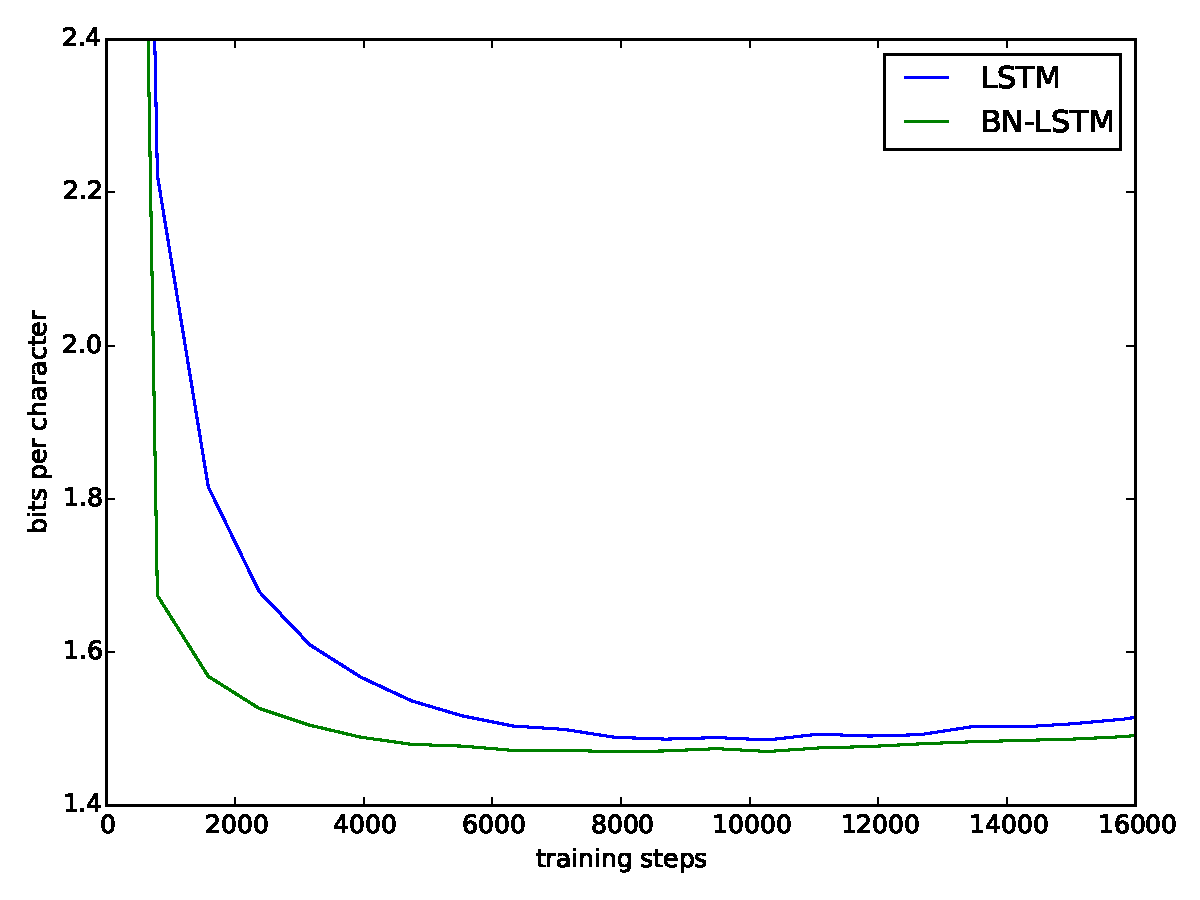
\includegraphics[width=7cm]{figures/ptb_valid.pdf}
%\caption{Bits-per-character on the validation set for Penn Treebank during training.}
%\label{fig:ptb_valid}
%\end{figure}
%
%\begin{table}
%\center
%\begin{tabular}{c|c}
%  \hline
%  LSTM & BN-LSTM\\
%  \hline
%  NaN & NaN\\
%  \textbf{NaN} & \textbf{NaN}\\
%\end{tabular}
%\caption{Bits-per-character on the Penn Treebank test string.}
%\label{tab:ptb_test}

\subsection{TIMIT}

[do we include this? I'm not opposed to it but not sure what to say]

\subsection{Teaching Machines to Read and Comprehend}

To demonstrate the generality and practical applicability of our
reparameterization, we take an implementation of the Attentive Reader
model~\cite{attentivereader} and simply replace the LSTM with our
BN-LSTM.
Additionally we try a variant where we also introduce batch
normalization into the attention computations, normalizing each term
going into the tanh nonlinearities.
Without any tweaking, we gain dramatic acceleration of training.

[Caglar will write a blurb on how the subset of data is selected]

[I will show training curves]

\section{Conclusion}

\bibliography{index}

\end{document}
